\documentclass[tikz]{standalone}

\usepackage{tikz}
\usetikzlibrary{trees}
\usetikzlibrary{shapes}
\usetikzlibrary{positioning}
\usetikzlibrary{arrows.meta}

\tikzset{
    pointer/.style = {thick,draw=black,triangle 45-*,shorten >=-3pt},
    cell/.style = {rectangle, thick, draw=black,minimum width = 1cm, minimum height =1.0cm,fill=yellow!20},
    mynode/.style = {circle, thick, draw=black, align=center,fill=yellow!40,font=\ttfamily\bfseries\Large},
    mynoder/.style = {circle, thick, draw=black, align=center,fill=red!30,font=\ttfamily\bfseries\Large},
    mynodeb/.style = {circle, thick, draw=black, align=center,fill=blue!30,font=\ttfamily\bfseries\Large},
    edgen/.style = {-latex,ultra thick},
    edger/.style = {-latex,ultra thick,red},
    edgeb/.style = {-latex,ultra thick,blue},
    edgeg/.style = {-latex,ultra thick,gray},
    edgegd/.style = {-latex,ultra thick,brown,dashed}, % back
    edgevd/.style = {-latex,ultra thick,violet,dotted}, % forward
    edgexd/.style = {-latex,ultra thick,blue,densely dotted}, % traversal
    every picture/.style={/utils/exec={\ttfamily\bfseries}},
    every picture/.style={font issue=\ttfamily\bfseries},
    font issue/.style={execute at begin picture={#1\selectfont}
  }
}

\newcommand{\R}[1]{\textcolor{red}{#1}}
\newcommand{\B}[1]{\textcolor{violet}{#1}}

\begin{document}

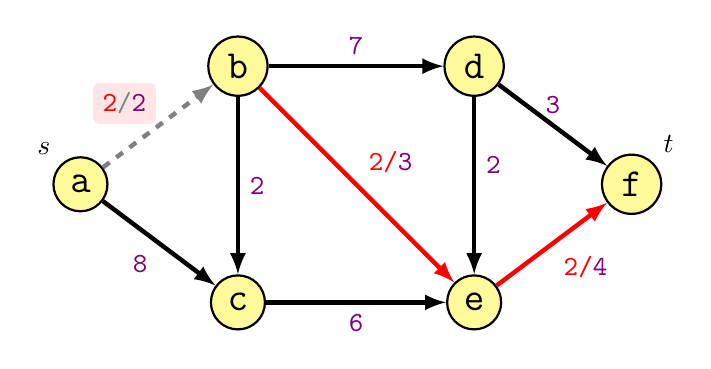
\begin{tikzpicture}[scale=1.00,transform shape]
\node[mynode, label={above left:$s$}] at (0.0, 1.5) (a) {a};
\node[mynode] at (2.0, 3.0) (b) {b};
\node[mynode] at (2.0, 0.0) (c) {c};
\node[mynode] at (5.0, 3.0) (d) {d};
\node[mynode] at (5.0, 0.0) (e) {e};
\node[mynode, label={above right:$t$}] at (7.0, 1.5) (f) {f};
%
\draw[edger] (a) edge[above left,color=gray,dashed] node[rounded corners=2pt,fill=red!10] {\R{2}/\B{2}} (b);
\draw[edgen] (b) edge[right] node {\B{2}} (c);
\draw[edgen] (a) edge[below left] node {\B{8}} (c);
\draw[edgen] (b) edge[above] node {\B{7}} (d);
\draw[edger] (b) edge[above right] node {\R{2}/\B{3}} (e);

\draw[edgen] (c) edge[below] node {\B{6}} (e);
\draw[edgen] (d) edge[above] node {\B{3}} (f);
\draw[edgen] (d) edge[above right] node {\B{2}} (e);
\draw[edger] (e) edge[below right] node {\R{2}/\B{4}} (f);
\end{tikzpicture}

\end{document}